
% [computermodern], 
% \documentclass[numbers]{sigplanconf}
\documentclass[10pt,preprint,twocolumn]{acmart}

\usepackage[T1]{fontenc}
\usepackage{libertine}%% Only as example for the romans/sans fonts
\usepackage[scaled=0.85]{beramono}

% \usepackage[utf8]{inputenc}
% \usepackage[russian,english]{babel}

\usepackage{url}
% \usepackage{code}
% \usepackage{cite}
\usepackage{amsmath}
\usepackage{amssymb}
\usepackage{graphicx}
\usepackage{chessboard}
\usepackage{gensymb}

% \usepackage{chessfs}
\usepackage{adjustbox}

% Define black versions of pieces for inline use. Gross, but it works.
\newcommand{\Pawn}[1][1.3ex]{%
\adjustbox{Trim=4.3pt 2.6pt 4.3pt 0pt,width=#1,margin=0.2ex 0ex 0.2ex 0ex}{\BlackPawnOnWhite}%
}%
\newcommand{\Rook}[1][1.58ex]{%
\adjustbox{Trim=3.2pt 2.2pt 3.2pt 0pt,width=#1,raise=0ex,margin=0.1ex 0ex 0.1ex 0ex}{\BlackRookOnWhite}%
}%
\newcommand{\Knight}[1][1.85ex]{%
\adjustbox{Trim=2.3pt 2.35pt 2.5pt 0pt,width=#1,raise=-0.03ex,margin=0.14ex 0ex 0.14ex 0ex}{\BlackKnightOnWhite}%
}%
\newcommand{\Bishop}[1][1.79ex]{%
\adjustbox{Trim=2.3pt 2pt 2.3pt 0pt,width=#1,raise=-0.12ex,margin=0.1ex 0ex 0.1ex 0ex}{\BlackBishopOnWhite}%
}%
\newcommand{\Queen}[1][2.05ex]{%
\adjustbox{Trim=1.2pt 2.2pt 1.2pt 0pt,width=#1,raise=-0.08ex,margin=0.1ex 0ex 0.1ex 0ex}{\BlackQueenOnWhite}%
}%
\newcommand{\King}[1][1.95ex]{%
\adjustbox{Trim=2pt 2pt 2pt 0pt,width=#1,raise=-0.06ex,margin=0.13ex 0ex 0.13ex 0ex}{\BlackKingOnWhite}%
}%

\interfootnotelinepenalty=0

% lets me explicitly set a. or 1. etc. as enum label
\usepackage{enumitem}

\pagestyle{empty}

\usepackage{ulem}
% go back to italics for emphasis, though
\normalem

\usepackage{natbib}

\setlength{\footnotesep}{2em}

% \newcommand\comment[1]{}
\newcommand\sfrac[2]{\!{}\,^{#1}\!/{}\!_{#2}}

% skip acm copyright shits
\makeatletter
\def\@copyrightspace{\relax}
\makeatother

\setcopyright{none}

\begin{document} 

% \copyrightyear{2019}

\acmConference{SIGBOVIK~2019}{April 1, 2019, Pittsburgh, Pennsylvania, USA}

\title[Elo World]{Elo World, a framework for \\ benchmarking weak chess \\ engines}
% \authorinfo{Dr.~Tom Murphy VII Ph.D.}{tom7.org Foundation}{tom7@tom7.org}
\author{Dr.~Tom Murphy VII Ph.D.}\email{tom7@tom7.org}
\thanks{Copyright \copyright\ 2019 the Regents of the Wikiplia Foundation.
Appears in SIGBOVIK 19119 with the
%
title inflation
%
of the Association for Computational Heresy; {\em IEEEEEE!}
press, Verlag-Verlag volume no.~0x40-2A. 1600 rating points}

\ccsdesc[500]{Evaluation methodologies~Tournaments}
\ccsdesc[500]{Chess~Being bad at it}
% \ccsdesc[100]{Software and its engineering~Control structures}
% \ccsdesc[300]{Theory of computation~Control primitives}

\keywords{pawn, horse, bishop, castle, queen, king}
% \keywords{chess, bad}

\setchessboard{showmover=false}

\newcommand\checkmate{\hspace{-.05em}\raisebox{.4ex}{\tiny\bf ++}}

\renewcommand\th{\ensuremath{{}^{\textrm{th}}}}
\newcommand\st{\ensuremath{{}^{\textrm{st}}}}
\newcommand\rd{\ensuremath{{}^{\textrm{rd}}}}
\newcommand\nd{\ensuremath{{}^{\textrm{nd}}}}
\newcommand\at{\ensuremath{\scriptstyle @}}

\date{1 April 2019}

\maketitle \thispagestyle{empty}

\section{Introduction}

Fiddly bits aside, it is a solved problem to maintain a numeric skill
rating of players for some game (for example chess, but also sports,
e-sports, probably also z-sports if that's a thing). Though it has
some competition (suggesting the need for a meta-rating system to
compare them), the Elo Rating System~\cite{elo1978rating} is a simple
and effective way to do it. This paper is concerned with Elo in chess,
its original purpose.

The gist of this system is to track a single score for each player.
The scores are defined such that the expected outcomes of games can be
computed from the scores (for example, a player with a rating of 2400
should win 9/10 of her games against a player with a rating of 2000).
If the true outcome (of e.g.~a tournament) doesn't match the expected
outcome, then both player's scores are adjusted towards values that
would have produced the expected result. Over time, scores thus become
a more accurate reflection of players' skill, while also allowing for
players to change skill level. This system is carefully described
elsewhere, so we can just leave it at that.

The players need not be human, and in fact this can facilitate running
many games and thereby getting arbitrarily accurate ratings.

The problem this paper is concerned with is that basically all chess
tournaments (whether with humans or computers or both) are between
players who know how to play chess, are interested in winning their
games, and have some reasonable level of skill. This makes it hard to
give a rating to weak players: They just lose every single game and so
tend towards a rating of $-\infty$\footnote{Some organizations don't
  even let ratings fall beneath a certain level, for example, the
  lowest possible USCF rating is 100.} Even if other comparatively
weak players existed to participate in the tournament and occasionally
lose to the player under study, it may still be difficult to
understand how this cohort performs in any absolute sense. (In
contrast we have ``the highest ever human rating was 2882,'' and
``there are 5,323 players with ratings in 2200--2299'' and ``Players
whose ratings drop below 1000 are listed on the next list as
'delisted'.''~\cite{fideratings}) It may also be the case that all
weak players always lose to all strong players, making it unclear just
how wide the performance gap between the two sets is. The goal of
this paper is to expand the dynamic range of chess ratings to span
all the way from extremely weak players to extremely strong ones, while
providing canonical reference points along the way.

\section{Elo world}

Elo World is a tournament with dozens of computer players. The
computer players include some traditional chess engines, but also many
algorithms chosen for their simplicity, as well as some designed to
be competitively bad.

The fun part is the various algorithms, so let's get into that. First,
some ground rules and guidelines:
\begin{itemize}
\item No resigning (forfeiting) or claiming a draw. The player will
  only be asked to make a move when there exists one, and it must
  choose a move in finite time. (In practice, most of the players are
  extremely fast, with the slowest ones using about one second of
  CPU time per move.)
\item The player can retain state for the game, and executes moves
  sequentially (for either the white or black pieces), but cannot have
  state meaningfully span games. For example, it is not permitted to
  do man-in-the-middle attacks~\cite{blind} or learn opponent's moves
  from previous rounds, or to get better at chess. The majority of
  players are actually completely stateless, just a function of type
  ${\tt position} \rightarrow {\tt move}$.
\item black and white behave the same
\item Avoid game-tree search. Minimax, alpha--beta, etc. are the
  correct way to play chess programmatically. They are well-studied
  (i.e., boring) and effective, and so not well suited to our problem.
  A less obvious issue is that they are endlessly parameterizable, for
  example the search ply; this leaves us with a million things to
  fiddle with. In any case, several traditional chess engines are
  included for comparison.
\end{itemize}

% dispense with alpha-beta, etc.

\subsection{Simple players}

\newcommand\describeplayer[1]{\smallskip\noindent {\texttt{\textbf{#1}}}.\ \ }
\newcommand\player[1]{\texttt{#1}}
\newcommand\russian{
  
\includegraphics[height=0.9em]{zazdarovye}
}
\newcommand\deterministic{
  
\includegraphics[height=0.9em]{deterministic}
}
\newcommand\traditional{
  
\includegraphics[height=0.9em]{traditional}
}
\newcommand\vegetarian{
  
\includegraphics[height=0.9em]{vegetarian}
}
\newcommand\canonical{
  
\includegraphics[height=0.9em]{canonical}
}
\newcommand\stateful{
  
\includegraphics[height=0.9em]{stateful}
}
\newcommand\asymmetric{
  
\includegraphics[height=0.9em]{asymmetric}
}

\describeplayer{random\_move} We must begin with the most canonical of all
strategies: Choosing a legal move uniformly at random. This is a
lovely choice for Elo World, for several reasons: It is simple to
describe. It is clearly canonical, in that anyone undertaking a
similar project would come up with the same thing. It is capable of
producing any sequence of moves, and thus completely spans the gamut
from the worst possible player to the best. If we run the tournament
long enough, it will eventually at least draw games even against a
hypothetical perfect opponent, a sort of Boltzmann Brilliancy. Note
that this strategy actually does keep state (the pseudorandom pool),
despite the admonition above. We can see this as not really state but
a simulation of an external source of ``true'' randomness. Most other
players fall back on making random moves to break ties or when their
primary strategy does not apply. \canonical

\describeplayer{same\_color} When playing as white, put pieces on
white squares. Vice versa for black. This is accomplished by counting
the number of white pieces on white squares {\em after} each possible
move, and then playing one of the moves that maximizes this number.
Ties are broken randomly. Like many algorithms described this way, it
tends to reach a plateau where the metric cannot be increased in a
single move, and then plays randomly along this local maximum
(Figure~\ref{fig:samecolor}). This particular strategy moves one
knight at most once (because they always change color when moving)
unless forced; on the other hand both bishops can be safely moved
anywhere when the metric is maxed out.

\begin{figure}[ht]
\chessboard[setfen=1n1r3q/1Q2r1bp/1p1p1p1n/p1pPp1p1/P1PkR3/1P1P1P1N/6BP/1N1R3K b - - 85 73,showmover=false]
\caption{\player{same\_color} (playing as white) checkmates
  \player{same\_color} (playing as black) on move 73. Note that since
  white opened with Nh3, the h2 pawn is stuck on a black square.
  Moving the knight out of the way would require that move to be
  forced. } \label{fig:samecolor}
\end{figure}

\describeplayer{opposite\_color} Same idea, opposite parity.

% XXX more clear/efficient description here?
\describeplayer{pacifist} Avoid moves that mate the opponent, and
failing that, avoid moves that check, and failing that, avoid moves
that capture pieces, and failing that, capture lower value pieces.
Break ties randomly. This is one of the worst strategies, drawing
against players that are not ambitious about normal chess pursuits,
and easily losing to simple strategies. On the other hand, it does
rarely get forced into mating its opponent by aggressive but weak
players. \vegetarian

\describeplayer{first\_move} Make the lexicographically first legal
move. The moves are ordered as $\langle\!$~\verb+src_row+,
\verb+src_col+, \verb+dst_row+, \verb+dst_col+,
\verb+promote_to+~$\!\rangle$ for white (rank $1$ is row $0$) and the rows
are reversed for black to make the strategy symmetric. Tends to
produce draws (by repetition), because knights and rooks can often
move back and forth on the first few files. \deterministic

\describeplayer{alphabetical} Make the alphabetically first move,
using standard PGN short notation. White and black both try to move
towards A1. \asymmetric \deterministic

\describeplayer{huddle} As white, make moves that minimize the total
distance between white pieces and the white king. Distance is the
Chebyshev distance, which is the number of moves a king takes to move
between squares. This forms a defensive wall around the king
(Figure~\ref{fig:huddle}).

\begin{figure}[ht]
\chessboard[setfen=2r4r/5n2/1p4p1/nP5p/1Ppk3P/2NPRNP1/1bRPPP2/2BQKB2 b - - 80 158,showmover=false]
\caption{\player{huddle} (white) checkmates \player{pacifist} on move
  158 with substantial help. Note that white's distal pawns have
  advanced; these are actually the same distance from the King as they
  would be in their home row, since the distance metric includes diagonal
  moves. } \label{fig:huddle}
\end{figure}

\describeplayer{swarm} Like \player{huddle}, but instead move pieces
such that they are close to opponent's king. This is essentially an
all-out attack with no planning, and manages to be one of the
better-performing ``simple'' strategies. From the bloodbaths it
creates, it even manages a few victories against strong opponents
(Figure~\ref{fig:swarm}).

% XXX illustrate the moves here
\begin{figure}[ht]
\chessboard[setfen=rnbqkb1r/pp1ppp1p/7p/1Bp5/3PnP2/8/PPP3PP/RN1QK1NR b KQkq - 1 5,showmover=false]
\caption{\player{swarm} (white) vs.~\player{stockfish1m\_r4096}
  with black to move after 1.~d4 Nf6 2.~Bh6 gxh6 3.~f4 c5 4.~e4 Nxe4
  5.~Bb5. Black blunders 5\ldots f6??, which must have been a random
  move as \player{swarm} immediately wins with 6.~Qh5++.} \label{fig:swarm}
\end{figure}

\describeplayer{generous} Move so as to maximize the number of
opponent moves that capture our pieces, weighting by the value of the
offered piece ($\pawn = 1$, $\bishop = \knight = 3$, $\rook = 5$,
$\queen = 9$). A piece that can be catpured multiple ways is counted
multiple times.

\describeplayer{no\_i\_insist} Like \player{generous}, but be overwhelmingly
polite by trying to {\em force} the opponent to accept the gift of material.
There are three tiers: Avoid at all costs mating the opponent (and moreso
checkmating). Stalemate is polite, but it is more canonical for two
polite players to form a draw by repetition, from continually offering up
material to one another and declining it. Next, avoid situations where
the opponent can refuse our gift; among these, prefer the move where the
opponent must capture the highest value piece. Finally, prefer moves
where the expected value of the offered material (i.e.~against random play)
is highest. (This means that if there are three moves, and one captures a
rook but the others capture nothing, the value is $5/3$.) This strategy
almost never wins, but is not among the worst players, since it often forces
a draw by exchanging all its pieces.

\describeplayer{reverse\_starting} This player thinks that the board is
upside-down, and as white, tries to put its pieces where black pieces
start. This often causes some conflict since the black pieces are already
there, but can also end peacefully (Figure~\ref{fig:reversestarting}).

\begin{figure}[ht]
\chessboard[setfen=1NB1K2R/8/8/8/8/8/6p1/rnbqkbn1 b - - 19 64,showmover=false]
\caption{\player{reverse\_starting} draws against itself
by repetition, both players having happily moved their surviving pieces into the
correct spots.} \label{fig:reversestarting}
\end{figure}

% TODO: Cyrillic tag or toast at the end
\describeplayer{cccp} Prioritize moves that Checkmate, Check, Capture
or Push, in that order. Push means to move pieces as deep as possible
into enemy territory (without any regard for their safety). Ties are
broken deterministically by the source/destination squares, so this
one is technically asymmetric.
% \begin{otherlanguage*}{russian}
% За здоровье!
% \end{otherlanguage*}
\deterministic \asymmetric \russian

\describeplayer{suicide\_king} Take a random move that minimizes the
distance between the two kings. Putting one's king out in the open is
very unprincipled (Figure~\ref{fig:cccpsuicide}), but it does produce
enough pressure to win against unambitious opponents.

\begin{figure}[ht]
  \chessboard[setfen=r1bq1bnr/pppp1p1p/2PQ4/8/2k6/8/PPP1PPPP/RN2KBNR b KQ - 0 7,showmover=false]
\caption{\player{suicide\_king} (black) dramatically failing against
  \player{cccp}'s slightly more principled play, after 1.~d4
  g5 2.~Bxg5 Nc6 3.~Bxe7 Kxe7 4.~d5 Kd6 5.~dxc6+ Kc5 6.~Qd6+ Kc4.
  White delivers a discovered mate with 7.~e4++.} \label{fig:cccpsuicide}
\end{figure}

\describeplayer{sym\_mirror\_y} As white, try to maximize symmetry
when flipping vertically. Zero penalty for opposing e.g.~a \King\, with
a \king, but a small penalty when the pieces are not the same type,
and a larger penalty when they are not opposite colors. The starting
position is already symmetric this way, so this usually has the effect
of copying the opponent's moves when possible. As ``copy your
opponent's moves'' is a common (but underspecified) strategy
discovered by many children, this player is close to being canonical.
However, it admits a bit too much arbitrary choice in the penalties
assigned.

\describeplayer{sym\_mirror\_x} As \player{sym\_mirror\_y}, but
maximize symmetry when flipping horizontally. This does not make much
chess sense, but can produce aesthetic arrangements.

\describeplayer{sym\_180} As \player{sym\_mirror\_y}, but maximize
symmetry under 180\degree\ rotation
of the board (Figure~\ref{fig:sym180}. An emergent priority is
to ``castle'' with the king and queen to ``fix'' them.

\begin{figure}
  \chessboard[setfen=2bkr3/8/n1r1pppp/1PppQ2P/N2BPPP1/1PPP1R1N/8/3RKB2 b - - 8 66,showmover=false]
  \caption{\player{sym\_180} (white) vs. \player{pacifist} after 66 moves. Note that the position is not quite rotationally symmetric, but is close given the material.} \label{fig:sym180}
\end{figure}

\describeplayer{min\_oppt\_moves} Take a move that minimizes the
number of resulting legal moves for the opponent, breaking ties
randomly. This is a beautifully simple approach that generalizes many
chess principles: Occupying space reduces the destination squares
available to the opponent; capturing their pieces reduces the number
of their pieces that they can move; pinning pieces or checking the
king further reduces the legal moves; and mating the opponent is the
best possible move.\footnote{However note that it does not distinguish
  checkmate and stalemate, despite these having very different
  results.} Among the players in the paper, this one is Pareto
efficient in terms of its simplicity and effectiveness. \canonical

\describeplayer{equalizer} Prefer to move a piece that has been
moved the fewest times, and then prefer moving to a square that
has been visited the fewest times. Castling counts as moving
both the king and rook, and visiting both destination squares.
This is the first strategy described that keeps meaningful state.
\canonical \stateful

\subsection{Fate-based players}

If we keep state, then we can track the location of each piece as it
moves around the board (allowing us to distinguish the two rooks, or
follow a pawn as it promotes). We can then use statistics on the
average fates of each piece over hundreds of millions of games to
guide the moves. These statistics give us, for each piece (e.g.~the c2
pawn) and square, how likely it is to end the game on that square, and
how likely it is to be alive or dead there when the game
ends~\cite{survival}.

\describeplayer{safe} This strategy moves pieces towards squares where
they are likely to end the game alive. For this strategy and several
others, simply moving to maximize this score (e.g.~its sum or product
over all pieces) is very boring, since the score is almost always
maximized in the starting position. So this strategy actually makes
each move randomly, weighted by the total score of the resulting
positions. The scores are normalized (with the lowest-scoring move
receiving weight 0.0 and the highest 1.0) and then sampled according
to these weights. Without normalization, the play is almost identical
to uniformly random, since the weights of the resulting positions tend
to be very similar (dominated by the many pieces that don't move). But
it's pretty arbitrary. \stateful

\describeplayer{popular} Like \player{safe}, but the score for a
piece/square pair is the probability that the piece ends on that
square, whether it lives or dies. This player likes to follow the
crowd! \stateful

\describeplayer{dangerous} The dual of \player{safe}; the score is the
probability that the piece dies on that square. Note that a king is
said to die if it is checkmated or his side resigns. This player likes
to live life on the edge! \stateful

\describeplayer{rare} The dual of \player{dangerous}; the score
is one minus the probability of ending the game on that square. This
player has a thirst for adventure! \stateful

\describeplayer{survivalist} Like the above, but the score is the
ratio of the survival and death probabilities on the square. In the
data set, every piece ends alive or dead in every square (except
for the bishops, which can only legally occupy squares of their
color) at least 1000 times, so each ratio is defined. Here, the
sums of ratios have plenty of variability, and the highest
ratios are not so often on the starting squares. So with this
strategy, we simply do a weighted sample from the moves according
to their (non-normalized) scores. \stateful

\describeplayer{fatalist} The dual of \player{survivalist}; the score is
the ratio of the death and survival probability on the square. This
player knows that even if you win, you just have to keep playing over
and over again, so you might as well get it over with! \stateful

\subsection{Engine-based players}

Of course, people have been making more serious attempts at automating
chess since before computers, and there are thousands of chess engines
out there. We include a few in here to represent the high end of
skill, and to make sure that weaker players are evaluated somewhat in
terms of their ability to play chess proper, not just beat other weak
players.

\describeplayer{stockfish0} Stockfish~\cite{stockfish} is probably the
strongest open-source chess engine (or even publicly available
engine); at full strength its play is estimated to be around 3500 Elo
on the FIDE scale. Aside from being quite machine-dependent (it can
search more moves in a given amount of time when it has a fast CPU
with many cores), there are many options to fiddle with. Stockfish can
use both opening books and endgame tables; neither is used here. It
also has a ``difficulty'' setting, which is set here to 0. Stockfish
is run in a separate process, and the board is reset before each move,
but I am not extremely hygienic about flushing e.g.~internal hash
tables between moves. One consequence of this attempt at statelessness
is that Stockfish sometimes walks into a draw by repetition in
positions where it would be able to win, because it doesn't know that
it is repeating positions. \traditional

% TODO: Does lichess publish the difficulty settings ? Nice to compare
% to my subjective skill level
\describeplayer{stockfish5} Stockfish as above, but at difficulty 5.
\traditional

\describeplayer{stockfish10} Same, at difficulty 10.
\traditional

\describeplayer{stockfish15} Same, at difficulty 15.
\traditional

\describeplayer{stockfish20} And difficulty 20, the maximum. Even
at this difficulty, Stockfish produces moves basically instantaneously.
\traditional

\describeplayer{stockfish1m} As expected, the engine's performance
increases steadily as the difficulty setting increases (without
apparently affecting the time to make moves). I don't know what it's
doing with these settings. The true way to unleash chess engines is to
give them a lot of CPU and memory to search. Since the tournament is
run simultaneously across about 60 threads\footnote{ The computer is
  the completely egregious AMD 2990WX ``Threadripper~2,'' which has 32
  cores (for 64 hardware threads) and 250 Watts of power dissipation
  at load. The torture of this CPU was part of the impetus for the
  paper.} using dozens of gigabytes of memory, and sometimes I would
play {\it Hollow Knight} while it ran, I wanted to avoid having the
performance be dependent on the scheduling environment. So here,
Stockfish is given a ``node'' budget of 1~million, hence {\sf 1m}. It
takes about one second per move when running alone, and is easily the
strongest player (type) evaluated.
\traditional

\begin{figure}[ht]
  \chessboard[setfen=r1bK1b2/1p1pn3/p2k3N/1np1pQ2/2P2P1P/N2P4/R5B1/4B2R w - - 1 37,showmover=false]
  \caption{\player{suicide\_king} (white) to move against
    \player{worstfish} after 36 moves. Since the kings
    are already at their minimum distance, white will make
    a move at random. 37.~Qxe5++ wins for white immediately,
    but \player{suicide\_king} plays 37.~Qxd7??. The only
    legal move is 37\ldots Bxd7++, so \player{worstfish}
    must play it, and thus wins one of its only victories.}
  \label{fig:worstfish}
% full game:
% 1. Nf3 g5 2. b4 Na6 3. Nxg5 Nc5 4. b5 f6
% 5. c4 Na6 6. Nf7 Rb8 7. d3 h6 8. Kd2 Nb4
% 9. Kc3 Rh7 10. Kd4 Rg7 11. Kc5 Nd5 12. Nxh6 Nb4
% 13. Na3 Rg3 14. Qc2 Bg7 15. f4 a6 16. Qb1 Bh8
% 17. Qb2 f5 18. Qf6 Rxg2 19. Qh4 Rxe2 20. Bg2 e5
% 21. Bd2 Bf6 22. Nf7 Bh8 23. Qf2 c6 24. Kd6 Re4
% 25. h4 Qc7+ 26. Kxc7 Nxa2 27. Raf1 c5 28. Nh6 Ke7
% 29. Qd4 Ke6 30. Rc1 Bg7 31. Be1 Ra8 32. Rc2 Nc3
% 33. Ra2 Ne7 34. Qxe4 Bf8 35. Kd8 Nxb5 36. Qxf5+ Kd6
% 37. Qxd7+ Bxd7++
\end{figure}

\describeplayer{worstfish} On the other hand, a strong chess engine
can also be used to play badly. When playing as white, for each legal
move, I ask Stockfish (configured as \player{stockfish0}) to evaluate
the resulting position from black's perspective.\footnote{By asking it
  to make a move, which also returns the evaluation of its move. The
  UCI protocol does not seem to offer a way to evaluate a position
  directly.} I then choose the move that produces the best position
for black. This is easily the worst player evaluated, but it is not
hard to imagine ways it could be worse. Indeed, a common twist on
chess is to play for a loss, called {\it Antichess} or {\it Losing
  Chess}~\cite{wikipedialosingchess}. Recently it was even proved that
white can always win (i.e.~lose)~\cite{watkins2017losing} in this
variant! However, the variant requires that you capture a piece if
you are able to, so strategies and engines that support this variant
cannot be directly applied.
We could use stronger settings of Stockfish, but since it already
invokes Stockfish for each legal move, it is also one of the slowest
players. Like Stockfish, it occasionally blunders an otherwise losing
position into a draw by repetition. But most importantly, its search
strategy when evaluating positions is not applying the correct logic
($\alpha$--$\beta$ pruning); it assumes that its opponent will choose
strong moves, and that it will itself play strong moves in future
plies. As a result, it sometimes allows the opponent to create a
situation where \player{worstfish} is forced to checkmate its opponent
(Figure~\ref{fig:worstfish}).

\describeplayer{topple10k} Topple~\cite{topple} is another strong
open source engine, provided to keep Stockfish on its toes. Here,
its node budget is 10,000. \traditional

\describeplayer{topple1m} Topple with a node budget of 1 million,
which like \player{stockfish1m} takes about one second per move.
Stockfish almost always wins, though it is not clear whether the
budgets are actually comparable. \traditional

\describeplayer{chessmaster.nes\_lv1} This is {\it Chessmaster} for
the Nintendo Entertainment System, published in AD 1989. Moves are
extracted from the game via emulation. This proved to be somewhat
delicate, because the in-memory representation of the board is not
that simple (it appears to be represented in two parallel arrays,
perhaps using the ``0x88 method'') and the game understandably goes
wild if you mess it up. To play a move, I restore a saved machine
state in the ``board editor'' mode, and then modify memory to contain
the desired board. I then emulate button presses to operate the game
menu and return to ``playing'' mode. Chessmaster repairs its internal
data structures from this board, and makes a move. During this time I
mash controller buttons to skip its dramatic tunes and modal messages
like \verb+CHECK+. Once some memory locations reach certain values,
the move has been played; I can diff the before and after boards to
uniquely determine the move. Since this approach uses emulation, it
would normally be completely deterministic, but I deliberately stall
for a random number of frames so that it can advance its internal
pseudorandom state. A nice thing about this engine is that it is an
earnest attempt at writing a good engine, but limited to the
techniques of the 1980s, and running on hardware that was underpowered
even for its day. It finishes well behind the modern engines, but
ahead of all the non-traditional strategies. \traditional

\describeplayer{chessmaster.nes\_lv2} Same as
\player{chessmaster.nes\_lv1}, but increasing the ``Level Of Play'' to
``Newcomer 2.'' Chessmaster has stronger levels still, but in these
modes it will think for several NES minutes, which takes multiple
seconds to emulate---too slow for our purposes. Still much
weaker than modern engines (Figure~\ref{fig:chessmaster}).
\traditional

\begin{figure}[ht]
  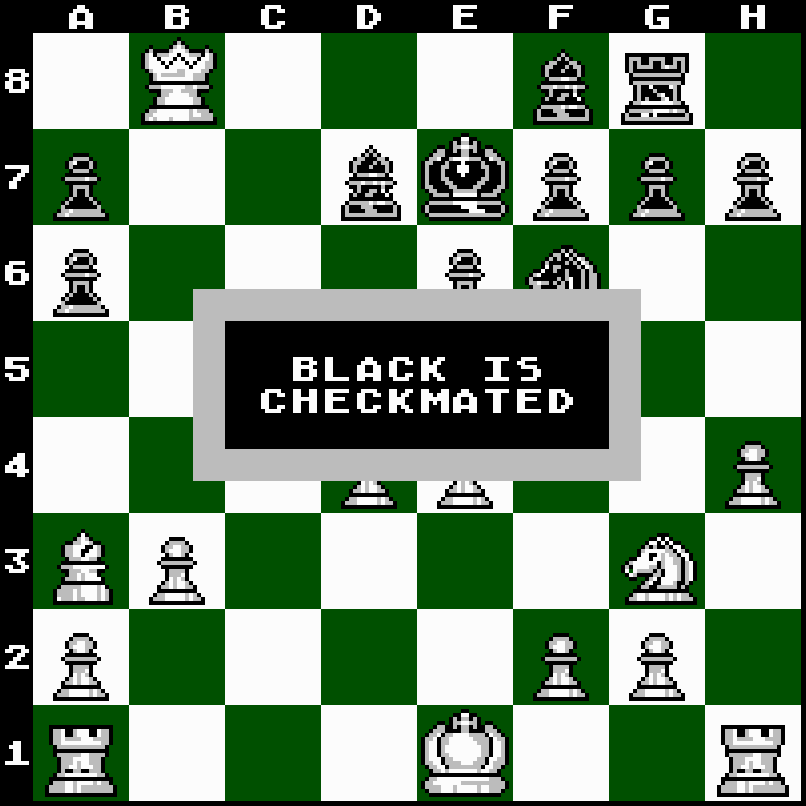
\includegraphics[width=0.75 \linewidth]{chessmaster}
  \caption{\player{stockfish1m} (2019; running on a modern machine) beats
    \player{chessmaster.nes\_lv2} (1989; running on an emulated NES)
    thousands of times without a loss or draw.} \label{fig:chessmaster}
\end{figure}

\subsection{Blind players}

\describeplayer{blind\_yolo} This player is only allowed to see the
64-bit mask of where pieces are placed on the board, but not their
colors or types. It is described in {\it Color- and Piece-blind
  Chess}~\cite{blind}.

\describeplayer{blind\_kings} As \player{blind\_yolo}, but forcing
the prediction to produce exactly one king for each side, which
improves its accuracy a little.

\describeplayer{blind\_spycheck} As \player{blind\_kings}, but
performing a ``spy check'' before each move. Here, the player tries
capturing each piece of a given (predicted) color with other pieces
of that same (predicted) color. If such a move is legal, then one
of the two pieces was mispredicted, so we prefer the capture over
sending an incorrect position to the engine.

Each of these uses a neural network to predict the configuration of
the board, and then the equivalent of \player{stockfish1m} to make a
move for that predicted board. (If that move is illegal because the
board was mispredicted, then it plays a random legal move.) These
players can therefore be seen as handicaps on \player{stockfish1m}.

\subsection{Diultion methods}

Even at its weakest setting, \player{stockfish0} crushes all of the
nontraditional strategies. This is not surprising, but it creates
a problem for quantifying their difference in skill (do they win
one in a million games? One in 10^{100}?). Having intermediate
players allows some Elo points to flow between the two tiers
transitively. One nice way to construct intermediate players is
by interpolation. We can interpolate between any two players,\footnote{
  Even if they are stateful! The interface separates ``please
  give me a move for the current state'' and ``the following
  move was played; please update your state,'' allowing them
  to disagree. So we can just keep two independent states for
  the two players.} but interpolating with the most canonical
player, \player{random\_move}. 


% Stockfish1m_32768 loses to reverse_starting in 3 moves!
1. e4 g5 2. Ba6 f5 3. Qh5


\describeplayer{stockfish1m\_r32768}
\describeplayer{stockfish1m\_r16384}
\describeplayer{stockfish1m\_r8192}
\describeplayer{stockfish1m\_r4096}
\describeplayer{stockfish1m\_r2048}
\describeplayer{stockfish1m\_r1024}
\describeplayer{stockfish1m\_r512}
\describeplayer{stockfish1m\_r256}
\describeplayer{stockfish1m\_r64}
\describeplayer{stockfish1m\_r128}

Ideally, such a system would be robust against adding new players,
but this is probably not the case.


% Names:
% "Stalemate"
% "Weaksauce"
% "back rank"
% "blunder"
% something with ..elo..   "elo world"
% inFIDElity
% blunderbuss
% 

Interpolation, like Scoville scale.


% miraculous win for "generous" strategy as black:
% playing against "suicide king". White forces black
% to mate him:
1. a4 b5 2. d3 Nh6 3. Kd2 Ng8 4. Kc3 Nh6
5. Kd4 c6 6. Ke5 f5 7. a5 Qb6 8. Bg5 Qe3+
9. Bxe3 Na6 10. f3 Nc5 11. Ra2 Ne4 12. f4 Nd2
13. Bf2 Nf3+ 14. exf3 Ng4+ 15. Kxf5 g5 16. Nh3 e5
17. Bh4 Ba3 18. b4 e4 19. Nf2 c5 20. c4 Ba6
21. g3 Rc8 22. Be2 Kf7 23. fxe4 d5 24. Qc1 dxe4
25. Rg1 bxc4 26. Rd1 cxd3 27. Qxc5 Rhf8 28. Nd2 Bc4
29. Kxg5 Rc7 30. Bf3 Ke8 31. Qe5+ Kf7 32. Qe6+ Kg7
33. Qb6 Rxf4 34. Nb3 Bb5 35. Qb7 d2 36. Nh3 Bc1
37. Qxa7 Be2 38. Nd4 h5 39. Ra1 Nf2 40. Raxc1 Nh1
41. Rf1 d1=Q 42. Qxc7+ Kh8 43. Kg6 Bc4 44. Bxd1 e3
45. Qf7 Bb3 46. Rf3 Nf2 47. Rc6 e2 48. Rc7 Rf5
49. Rc4 Rf4 50. Nb5 e1=Q 51. Rc2 Qc3 52. g4 Rf5
53. Ng1 Qc7 54. Rcc3 Nd3 55. Rc5 Nf2 56. Nc3 Ba2
57. Qh7+



% Fate-based algorithms.
% The deterministic version is fairly boring, since the
% highest probability states are similar to the starting
% position (this might not be true for "survivalist"
% or "fatalist"? check?)

% weighted random is almost the same as random, because
% the weights tend to be very similar when treated
% additively. They perform slightly different from
% random, as so (101.5 million games):

%  player	elo	w/l/d
%  dangerous	986.29	1374577/1501526/15683897
%  popular	997.34	1360053/1502995/15696952
%  random_move	1000.79	1540798/1337668/15681534
%  rare	1005.85	1554600/1326707/15678693
%  safe	1009.72	1341030/1502162/15716808

% then with normalization:
%  player	elo	w/l/d
%  popular	990.93	25756/43561/346683
%  safe	993.49	28082/40769/347149
%  dangerous	996.60	30063/37451/348486
%  rare	1005.82	50656/27390/337954
%  random_move	1013.15	41747/27133/347120


// Good site for some computer chess programs with ELO:
// http://www.computerchess.org.uk/ccrl/404/

\section{Conclusion}

Shout out to the Thursd'z Institute and anonymous commenters
on my blog for discussion of players and suggestions. Several
ideas were suggested by multiple people, increasing my confidence
that they are somehow canonical.

The author would like to thank the anonymous referees
of the Special Interest Group on
B
O
V
In
Chess journal for their careful reviews.

\nocite{elo1978rating}
\nocite{topple}
// citation for knights distance:
\nocite{miller2013counting}
\nocite{watkins2017losing}

% \balance
% \bibliographystyle{plain}
\bibliographystyle{ACM-Reference-Format}
\bibliography{chess}

\end{document}
